%%%%%%%%%%%%%%%%%%%%%%%%%%%%%%%%%%%%%%%%%%%%%%%%%%%%%%%%%%%%%%%%%%%%
%           Auteur :  P.TRAN BA, E.BOUTTIER                        %
%         Création :  08/06/2012 18:05                             %
%%%%%%%%%%%%%%%%%%%%%%%%%%%%%%%%%%%%%%%%%%%%%%%%%%%%%%%%%%%%%%%%%%%%

\documentclass[a4paper,11pt]{article}

% \usepackage[utf8]{inputenc}
% \usepackage[T1]{fontenc}
% %\usepackage{xunicode}
% \usepackage{fontspec}
% \defaultfontfeatures{Mapping=tex-text,Scale=MatchLowercase}
% \usepackage{a4wide}
% \usepackage{verbatim}
% %\usepackage{polyglossia}
% %\setdefaultlanguage{french}
% %~ \usepackage{listings}
% \usepackage[french]{babel}
% %~ \usepackage{url}
% %~ \usepackage{times}
% %\usepackage{minted}
% \usepackage{graphicx}
% %\input{graphviz}
\usepackage{xcolor,times}

\usepackage{listings}
  \newcommand*\styleC{\fontsize{9}{10pt}\usefont{T1}{ptm}{m}{n}\selectfont }
  \newcommand*\styleD{\fontsize{9}{10pt}\usefont{OT1}{pag}{m}{n}\selectfont }

  \makeatletter
  % on fixe le langage utilisé
  \lstset{language=matlab}
  \edef\Motscle{emph={\lst@keywords}}
  \expandafter\lstset\expandafter{%
    \Motscle}
  \makeatother


  \definecolor{Ggris}{rgb}{0.45,0.48,0.45}

  \lstset{emphstyle=\rmfamily\color{blue}, % les mots réservés de matlab en bleu
  basicstyle=\styleC,
  keywordstyle=\ttfamily,
  commentstyle=\color{Ggris}\styleD, % commentaire en gris
  numberstyle=\tiny\color{red},
  numbers=left,
  numbersep=10pt,
  lineskip=0.7pt,
  showstringspaces=false}
  %  % inclure le fichier source
  \newcommand{\FSource}[1]{%
  \lstinputlisting[texcl=true]{#1}
  }

  %%%%%%%%%
  \textwidth=15cm
  \textheight=21cm
  %\hoffset=-2.5cm
  \tolerance=9000
  \hbadness=9000
  \pretolerance=2500

\usepackage{pack_roman}

\usepackage{geometry}
\geometry{hmargin=2.5cm,vmargin=1.5cm}

\title{Projet de Traitement du Signal\\Segmentation d'image SAR\\Rapport}
\author{P.TRAN BA \& E.BOUTTIER}
\date\today

\begin{document}

\maketitle

\vspace{2cm}

\begin{abstract}

This report deals with a way to detect the edge using the normalized Ratio Of Exponentially Weighted Average (ROEWA) on opposite sides of the central pixel. It thus produces a map of edge with their intensity. In order to improve the result, it can be use in both direction horizontal and vertical, and the magnitude of the two components yields an edge strength map.

This edge detector can cope with the presence of speckle, which can be modeled as a strong multiplicative noise. So, It should be used for instance on SAR image. This report describe step by step the processus used in order to simulate a segmentation with MatLab.

\end{abstract}

\vspace{1cm}

\begin{abstract}

    Ce rapport traite d'une méthode de détection de rupture utilisant le rapport des moyennes pondérées exponentiellement (ROEWA) normalisé sur chaque côté d'un pixel central. Elle permet ainsi d'obtenir une carte des ruptures en intensité. Pour améliorer son efficacité, le processus peut-être appliqué suivant plusieurs directions, par exemple horizontalement et verticalement, les différentes composantes étant ensuite moyennées quadratiquement.

    Ce détecteur de rupture est particulièrement adapté pour traiter les signaux avec présence de bruit speckle multiplicatif, tel que les images radars à synthèse d'ouverture (Synthetic Aperture Radar — SAR). Ce rapport décrit étape par étape la simulation d'une segmentation sous MaltLab.

\end{abstract}

\newpage

\tableofcontents

\newpage

\section{Introduction}
\subsection{Préface}

En analyse d'images, la segmentation est une étape essentielle, préliminaire a des traitements de haut niveau tels que la classification, la détection ou l'extraction d'objets. Elle consiste à décomposer une image en régions homogènes. Les deux principales approches sont l'approche région et l'approche contour. L'approche région cherche à regrouper les pixels présentant des propriétés communes tandis que l'approche contour vise à détecter les transitions entre régions. Des détecteurs efficaces ont été développés dans le cadre de l'imagerie optique, mais s'avèrent inadaptés aux images SAR de par la présence d'un bruit speckle multiplicatif.

\subsection{Objectif du projet}

L'objectif de ce projet est d'effectuer la segmentation d'une image radar a synthèse
d'ouverture (image SAR) à l'aide d'une méthode originale de détection de
ruptures appliquée successivement sur les lignes et colonnes de l'image. La méthode
est issue d'une publication intitulée “An Optimal Multiedge Detector for SAR Image
Segmentation” publiée en mai 1998 dans la revue IEEE Transactions on Geoscience
and Remote Sensing.

\newpage

\section{Génération d'une ligne d'image SAR}

Cette partie consiste a générer des lignes d'image radar conformément au
modèle proposée par l'article. La méthode de segmentation choisie sera
d'abord testée sur ces lignes avant d'être appliquée a des images entières.

\subsection{Ligne d'image non bruitée R(x)}

Une ligne d'image apparaît comme une juxtaposition de segments de réflectivité constante.
Elle est correctement modélisée comme un processus constant par morceaux dont les
sauts d'intensité obéissent a un processus de Poisson de paramètre $\lambda$. La
largeur des segments obéit alors à une loi exponentielle de paramètre $\lambda$, $\frac{1}{\lambda}$ représentant
le nombre moyen de pixels séparant deux sauts d'intensité. On utilise donc le code MatLab suivant afin de générer une ligne d'image non bruitée avec 255.

\vspace{0.5cm}

\FSource{matlab/1.m}

\vspace{0.5cm}

\includegraphics[width=15cm]{capture/ergodicité.JPG}

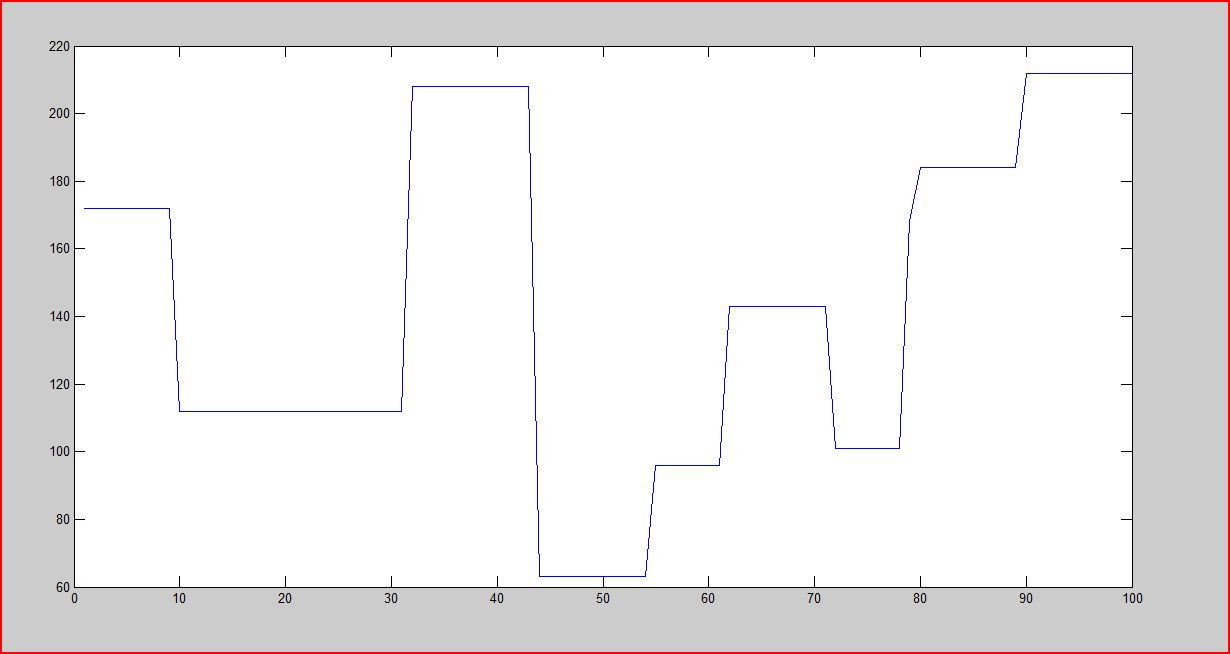
\includegraphics[width=15cm]{capture/Capturer.JPG}

\subsection{Bruit Speckle Multiplicatif n(x)}

Pour modéliser le bruit speckle, on utilisera une suite de variables aléatoires indépendantes suivant une loi Gamma de moyenne $\mu_n$ = 1 et de variance $\sigma_n^2$ = 1/L, où L correspond au nombre de vue moyennée.

\vspace{0.5cm}

\FSource{matlab/2.m}

\vspace{0.5cm}

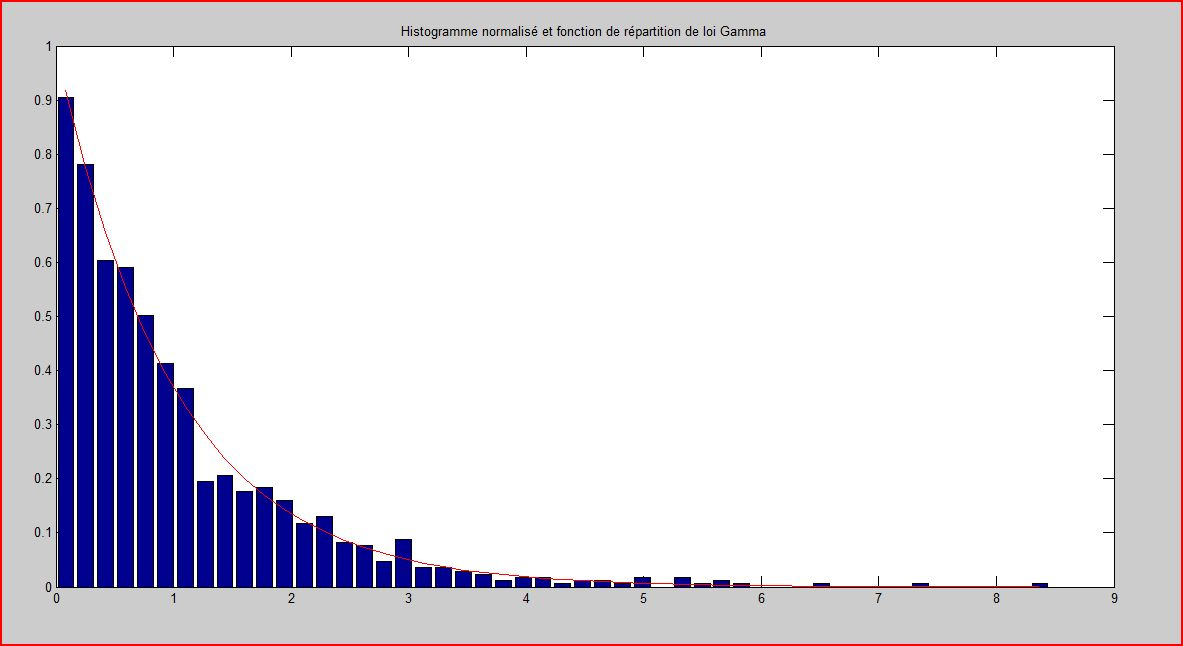
\includegraphics[width=15cm]{capture/bruit.JPG}

\subsection{Ligne d'image bruitée I(x)}

Pour obtenir une ligne d'image altérée par une bruit multiplicatif, il suffit de multiplier la ligne d'image et le bruit. Soit :
I(x) = R(x) * n(x).

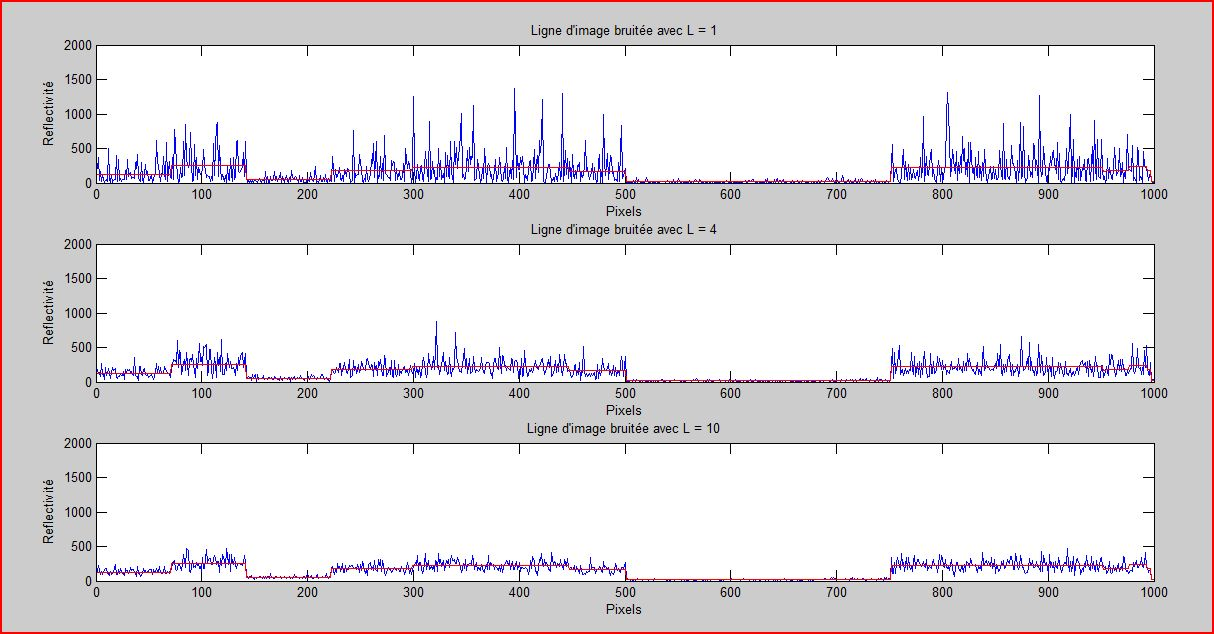
\includegraphics[width=15cm]{capture/ligne.JPG}

\newpage

\section{Analyse Spectrale d'une ligne d'image SAR}

Dans cette partie, le signal synthétique est étudié à l'aide des outils classiques d'analyse spectrale (corrélogramme, périodogramme).

\subsection{Périodogramme}

% TODO Figures à revoir

\vspace{0.5cm}

\FSource{matlab/3.m}

\vspace{0.5cm}

\subsection{Périodogramme cumulé}

% TODO Figures à revoir

\vspace{0.5cm}

\FSource{matlab/4.m}

\vspace{0.5cm}

\subsection{Corrélogramme}

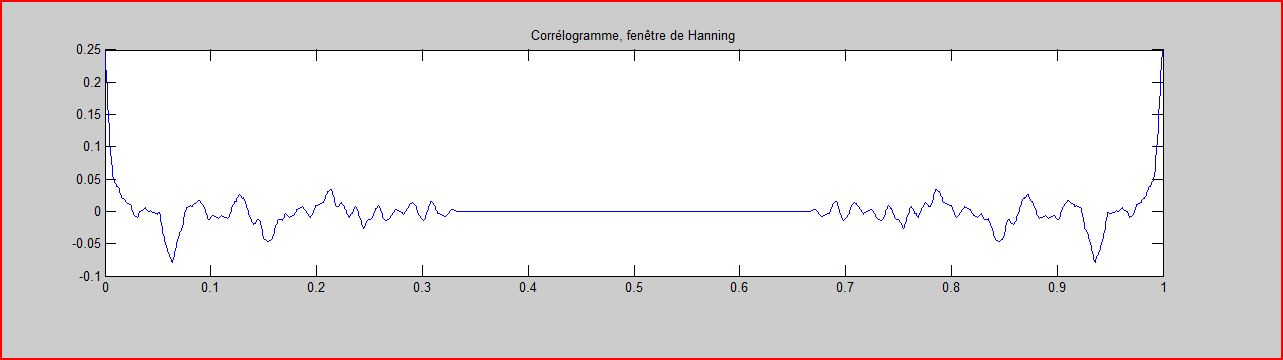
\includegraphics[width=15cm]{capture/correlo.JPG}

\vspace{0.5cm}

\FSource{matlab/5.m}

\vspace{0.5cm}

\newpage

\section{Détection de Ruptures sur une ligne d'image SAR}

Le détecteur ROEWA est appliqué au signal simulé. Il est basé sur des contrastes locaux
de niveau radiométrique moyen.

La détection s'effectue au moyen d'une fenêtre d'analyse glissante. Une forte différence
de réflectivité moyenne de part et d'autre d'un pixel permet de repérer un contour. Cette
méthode, bien adaptée aux images optiques, est mise en défaut pour l'imagerie radar.
La présence d'un bruit multiplicatif augmente en effet le taux de fausses détections
dans les régions de forte réflectivité. Pour pallier cette limitation, l'article propose
un détecteur basé non plus sur des différences, mais sur des rapports de réflectivité
moyenne. En outre, les moyennes arithmétiques sont remplacées par des moyennes
pondérées exponentiellement pour traiter les cas de contours multiples (présence de
plusieurs contours dans la fenêtre d'analyse). Les plus proches voisins du pixel central sont 
ainsi favorisés aux dépens de pixels plus éloignés pouvant correspondre a un
nouveau contour.

Le code MatLab ci dessous nous permet de synthétiser un filtre ISEF et de l'utiliser sur une
ligne bruitée.

\vspace{0.5cm}

\FSource{matlab/6.m}

\vspace{0.5cm}

% TODO image resultat
% TODO explication

Grâce au filtre ISEF, le bruit est fortement atténué et le signale est bien plus lisible. Nous allons donc pouvoir procéder à la détection de rupture par l'opérateur ROEWA noté $r_{max}$. Nous utilisons donc la suite du programme suivante afin de calculer le tableau des ROEWA :

\vspace{0.5cm}

\FSource{matlab/7.m}

\vspace{0.5cm}

Enfin, pour terminer, nous déterminons les ruptures à partir d'un seuil de ROEWA. Nous affichons suite au programme MatLab une figure présentant ROEWA, les ruptures détectées ainsi que le signal non bruité.

\vspace{0.5cm}

\FSource{matlab/8.m}

\vspace{0.5cm}

% TODO image resultat

\newpage

\section{Détection de Ruptures sur une image TEST}

La segmentation d'une image est réalisée en plusieurs étapes. Les ruptures sont détectés
successivement en ligne et en colonne de façon a créer une carte des contours délimitant
les régions de radiométrie différente.

La détection de contours sur une image est réalisée en deux temps. Le détecteur
ROEWA est d'abord appliqué successivement a chaque ligne de l'image, préalablement
lissée dans la direction opposée, pour obtenir la carte horizontale des contours $r_X (x, y)$.
En opérant de façon similaire dans la direction verticale, la carte verticale des contours
est construite. Ces deux composantes peuvent alors être combinées pour former la carte
des contours en deux dimensions : $r_{2D}(x,y)=\sqrt{{r^2}_X+{r^2}_Y}$

% TODO code matlab
% TODO bourge

\newpage

\section{Conclusion}

\end{document}
